\documentclass[a4paper]{amsbook}

\title{\textbf{Melbourne High School Maths Extension Group 2023 Handouts}}
\author{Nathan Wong\and Tom Yan}
%\dedicatory{Dedication}
\date{As of \today}
\usepackage[pass,a4paper]{geometry}
\usepackage[pdfusetitle]{hyperref}
\usepackage{pdfpages}
\setcounter{secnumdepth}{0}

\newcommand{\epigraph}[2]{%
\newpage \vspace*{8cm}
\thispagestyle{empty}
  \begin{quote}
	  {	
    \emph{#1}
    \begin{flushright}---{#2}
    \end{flushright}}
  \end{quote}}

\begin{document}
\maketitle
\newpage \vspace*{8cm}
\thispagestyle{empty}
\begin{center}
	  \emph{For Harold}
\end{center}
\epigraph{Thou, Nature, art my goddess. To thy law\\
My services are bound.}{W. Shakespeare, \emph{King Lear} (1606)}
\chapter*{Preface}
This book is a collection of MEG's published
materials this year. 
It is divided into two parts.
The first consists of MEG's weekly handouts
that were usually given out each meeting.
Each handout is hyperlinked in the table of contents.
All solutions that were published are
at the end of the section; however, the individual
solution documents have not been linked from the table
of contents. Moreover, solutions are not provided
for every problem that appears in the handouts,
as many have come from past competitions, and the official
solutions can be consulted.
When a problem is from a past competition, it is indicated
next to the question number for handouts from term 1, in the margin
for handouts from term 2 and onwards.

The second part consists of materials for this year's inaugral
SEHS maths games day. Included
are the problems and complete solutions for the problem
solving section, problems and answers for the relay.

This document has been produced by splicing together
individual digital copies of the source materials.
As such, naturally disregard any page numbers in any
of the individual documents. The hyperlinked table of contents
provides easy access to each section of the book.
\tableofcontents
\epigraph{ When I have clarified and exhausted a subject,
then I turn away from it, in order to go into darkness again;
the never-satisfied man is so strange if he has completed a structure,
then it is not in order to dwell in it peacefully, but in order to begin another.
I imagine the world conqueror must feel thus, who,
after one kingdom is scarcely conquered, stretches out his arms for others.}{%
	C.~F.~Gauss}
\part{Weekly handouts}

\phantomsection\addcontentsline{toc}{chapter}{Term 1}
\phantomsection\addcontentsline{toc}{section}{Term 1 Week 5: First Meeting}
\includepdf[pages=-]{../handouts/MEG_2023_First_Meeting_problems.pdf}
\phantomsection\addcontentsline{toc}{section}{Term 1 Week 7}
\includepdf[pages=-]{../handouts/MEG_2023_T1W7_Handout.pdf}
\phantomsection\addcontentsline{toc}{section}{Term 1 Week 8}
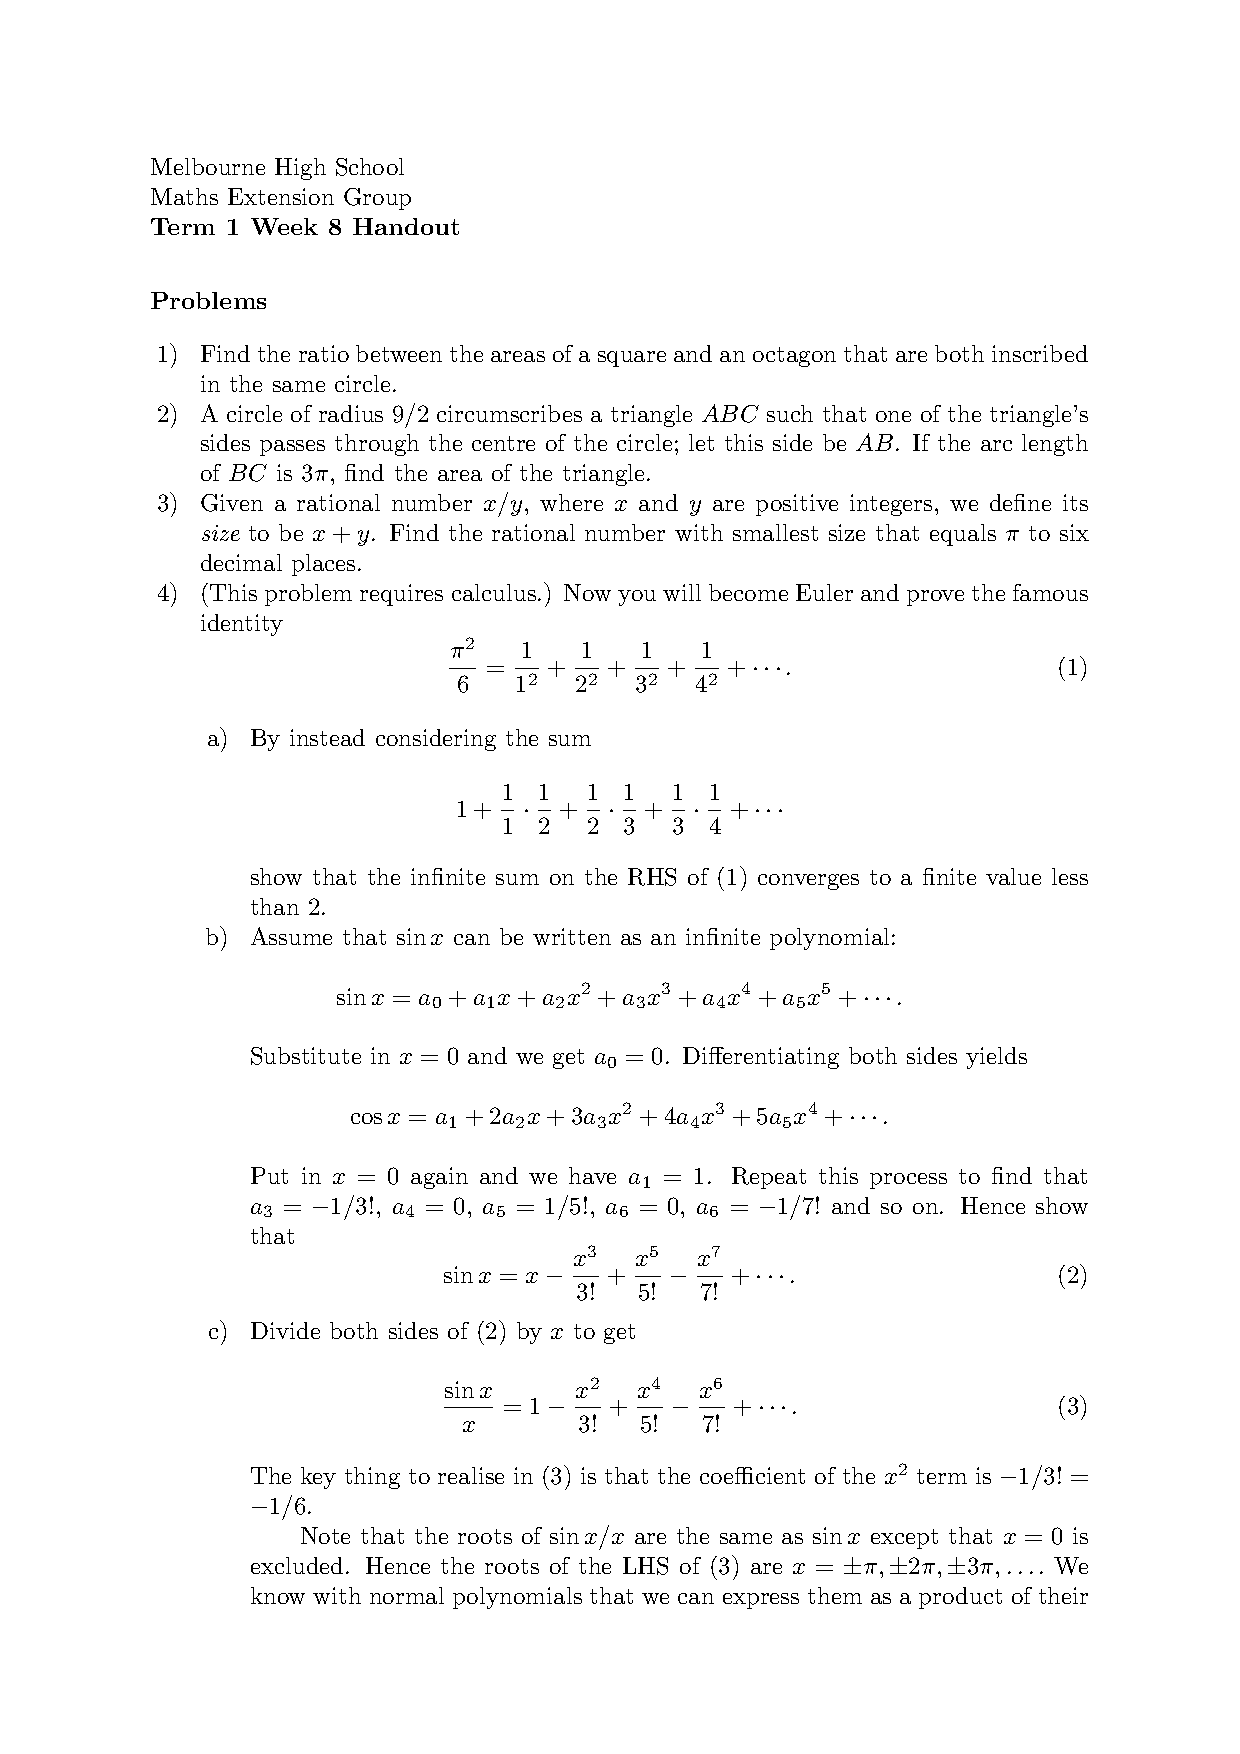
\includepdf[pages=-]{../handouts/MEG_2023_T1W8_Pi_Day_Handout.pdf}
%\includepdf[pages=-]{../handouts/MEG_2023_T1W8_Pi_Day.pdf}
\phantomsection\addcontentsline{toc}{section}{Term 1 Week 9}
\includepdf[pages=-]{../handouts/MEG_2023_T1W9_Handout.pdf}
\phantomsection\addcontentsline{toc}{section}{Term 1 Week 10}
\includepdf[pages=-]{../handouts/MEG_2023_T1W10_Handout.pdf}
\phantomsection\addcontentsline{toc}{section}{Term 1 Holidays}
\includepdf[pages=-]{../handouts/MEG_2023_T1_Holidays_Problems.pdf}
\phantomsection\addcontentsline{toc}{section}{April 15}
\includepdf[pages=-]{../handouts/MEG_2023_Euler_Gems.pdf}

\phantomsection\addcontentsline{toc}{chapter}{Term 2}
\phantomsection\addcontentsline{toc}{section}{Term 2 Week 5}
\includepdf[pages=-]{../handouts/MEG_2023_T2W5_Handout.pdf}
\phantomsection\addcontentsline{toc}{section}{Term 2 Week 6}
\includepdf[pages=-]{../handouts/MEG_2023_T2W6_Handout.pdf}
\phantomsection\addcontentsline{toc}{section}{Term 2 Week 7}
\includepdf[pages=-]{../handouts/MEG_2023_T2W7_Handout.pdf}
\phantomsection\addcontentsline{toc}{section}{Term 2 Holidays}
\includepdf[pages=-]{../handouts/MEG_2023_T2_Holidays_Problems.pdf}

\phantomsection\addcontentsline{toc}{chapter}{Term 3}
\phantomsection\addcontentsline{toc}{section}{Term 3 Week 4}
\includepdf[pages=-]{../handouts/MEG_2023_T3W4_Handout.pdf}
\phantomsection\addcontentsline{toc}{section}{Term 3 Week 5}
\includepdf[pages=-]{../handouts/MEG_2023_T3W5_Handout.pdf}
\phantomsection\addcontentsline{toc}{section}{Term 3 Week 6}
\includepdf[pages=-]{../handouts/MEG_2023_T3W6_Handout.pdf}
\phantomsection\addcontentsline{toc}{section}{Term 3 Week 8}
\includepdf[pages=-]{../handouts/MEG_2023_T3W8_Handout.pdf}
\phantomsection\addcontentsline{toc}{section}{Term 3 Week 9}
\includepdf[pages=-]{../handouts/MEG_2023_T3W9_Handout.pdf}
\phantomsection\addcontentsline{toc}{section}{Term 3 Holidays}
\includepdf[pages=-]{../handouts/MEG_2023_T3_Holidays_Handout.pdf}

\phantomsection\addcontentsline{toc}{chapter}{Term 4}
\phantomsection\addcontentsline{toc}{section}{Term 4 Week 2}
\includepdf[pages=-]{../handouts/MEG_2023_T4W2_Handout.pdf}
\phantomsection\addcontentsline{toc}{section}{Term 4 Week 3}
\includepdf[pages=-]{../handouts/MEG_2023_T4W3_Handout.pdf}

\phantomsection\addcontentsline{toc}{chapter}{Selected Solutions}
\includepdf[pages=-]{../handouts/solutions/MEG_2023_First_Meeting_Problems_Solutions.pdf}
\includepdf[pages=-]{../handouts/solutions/MEG_2023_T1W7_Handout_Solutions.pdf}
\includepdf[pages=-]{../handouts/solutions/MEG_2023_T1W8_Pi_Day_Handout_Solutions.pdf}
\includepdf[pages=-]{../handouts/solutions/MEG_2023_T1W9_Handout_Solutions.pdf}
\includepdf[pages=-]{../handouts/solutions/MEG_2023_T1W10_Handout_Solutions.pdf}
\includepdf[pages=-]{../handouts/solutions/MEG_2023_T1_Holidays_Problems_Solutions.pdf}
\includepdf[pages=-]{../handouts/solutions/MEG_2023_Euler_Gems_Solutions.pdf}
\includepdf[pages=-]{../handouts/solutions/MEG_2023_T2W5_Handout_Solutions.pdf}
\includepdf[pages=-]{../handouts/solutions/MEG_2023_T2W6_Handout_Solutions.pdf}
\includepdf[pages=-]{../handouts/solutions/MEG_2023_T2W7_Handout_Solutions.pdf}
\includepdf[pages=-]{../handouts/solutions/MEG_2023_T3W4_Handout_Solutions.pdf}
\includepdf[pages=-]{../handouts/solutions/MEG_2023_T3W5_Handout_Solutions.pdf}
\includepdf[pages=-]{../handouts/solutions/MEG_2023_T3W6_Handout_Solutions.pdf}
\includepdf[pages=-]{../handouts/solutions/MEG_2023_T3W8_Handout_Solutions.pdf}
\includepdf[pages=-]{../handouts/solutions/MEG_2023_T3W9_Handout_Solutions.pdf}
\includepdf[pages=-]{../handouts/solutions/MEG_2023_T3_Holidays_Handout_Solutions.pdf}
\includepdf[pages=-]{../handouts/solutions/MEG_2023_T4W2_Handout_Solutions.pdf}
\includepdf[pages=-]{../handouts/solutions/MEG_2023_T4W3_Handout_Solutions.pdf}
\epigraph{The case for my life, then, or for that of any one else
who has been a mathematician in the same sense in which I have been one,
is this: that I have added something to knowledge, and helped others to add more;
and that these somethings have a value which differs in degree only, and not
in kind, from that of the creations of the greatest mathematicians, or
of any of the other artists, great or small, who have left some kind
of memorial behind them.}{G.~H.~Hardy}
\part{SEHS Maths Games Day}
\phantomsection\addcontentsline{toc}{chapter}{Problem Solving}
\phantomsection\addcontentsline{toc}{section}{Problems}
\includepdf[pages=-]{../sehs_final/SEHS_Maths_Games_Day_2023_Problem_Solving.pdf}
\phantomsection\addcontentsline{toc}{section}{Solutions}
\includepdf[pages=-]{../sehs_final/SEHS_Maths_Games_Day_2023_Problem_Solving_Solutions.pdf}
\phantomsection\addcontentsline{toc}{chapter}{Relay}
\includepdf[pages=-]{../sehs_final/SEHS_Maths_Games_Day_2023_Running_Race_Problems.pdf}
% \phantomsection\addcontentsline{toc}{chapter}{Experimental and Creative Mathematics: Appendix}
% \includepdf[pages=-]{../sehs_final/SEHS_Maths_Games_Day_2023_Experimental_and_Creative_Mathematics_Appendix.pdf}

\end{document}
